\section*{Abstract}
This includes a demo of a Supplementary Figure, the \textit{narrow mode} which works for Figures and Supplementary Figure and use a chapter-specific citation.

\noindent{\bf Keywords:} Key1, Key2, Key3.

\begin{multicols}{2}
\section{Introduction}
\noindent
Here again, we showcase some old stuff that needs a (chapter-specific) citation \citepam{Darwin1859}.
Also, note the slight variation in referencing Supplementary Figures (\figrefS{fig:c1s1}) using \texttt{$\backslash$figrefS\{\}} (vs. \texttt{$\backslash$figref\{\}}).
Then again, it is time for dummy text: 

\section{A section}
% demo of a supplementary figure (in "narrow mode" )
\begin{supplFigure*}[!t]
\floatbox[{\capbeside\thisfloatsetup{capbesideposition={left,center},capbesidewidth=.5\fwidth}}]{supplFigure}[\FBwidth]
{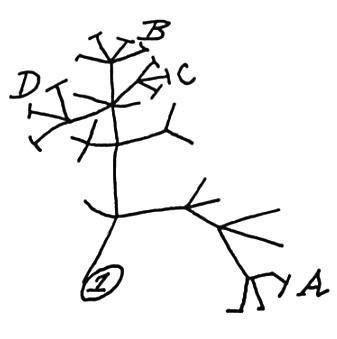
\includegraphics[width = .5\fwidth]{figures/c1/tree.jpg}}
{\caption[Darwins tree]{\label{fig:c1s1}\textbf{Darwins tree.}
Oh, the fame...}}
\end{supplFigure*}

\lipsum[2-4]

\bibliographystyleam{apalike}
\bibliographyam{library/c1.bib}
\end{multicols}